\documentclass[12pt]{article}

\usepackage{sbc-template}
\usepackage[utf8]{inputenc}
\usepackage[T1]{fontenc}
\usepackage[english,brazilian]{babel}
\usepackage{graphicx,url}
\usepackage{booktabs}
\usepackage{tikz}
\usetikzlibrary{arrows.meta,positioning}

\sloppy
\hyphenation{SMILES}

\title{Classificação de alvos proteicos a partir de descritores moleculares do ChEMBL com árvores de decisão}

\author{Bernan R. do Nascimento\inst{1}, Paulo E. R. Araujo\inst{1}, Thiago R. P. de Carvalho\inst{1}}

\address{Universidade Federal do Piauí (UFPI)\\
  Programa de Pós-Graduação em Ciência da Computação -- Teresina -- PI -- Brasil\\
  PPGCC010 -- Aprendizagem de Máquina (2026.2) -- Prof. Vinicius Ponte Machado
  \email{bernanr7@gmail.com, pauloaraujo@ufpi.edu.br}
  \email{thiago.rafael.pc@gmail.com}
}

\begin{document}

\maketitle

\begin{abstract}
  Predicting which protein target an active molecule acts on is an early step in drug discovery.
  We rebuild a dataset of 27,714 molecules active against four targets (EGFR, BACE1, DRD2 and HDAC1)
  from the ChEMBL 37 API and train a decision tree on five physicochemical descriptors and twelve
  counts taken from the SMILES string. With a grouped split, the SMILES counts raise accuracy from
  0.77 to 0.89 (mean of 10 seeds). A random split overestimates accuracy by 1.3 to 4.1 points,
  because a quarter of the test molecules have a twin with identical descriptors in the training set.
\end{abstract}

\begin{resumo}
  Prever em qual proteína-alvo uma molécula ativa age é uma etapa inicial da descoberta de
  fármacos. Reconstruímos pela API do ChEMBL 37 uma base de 27.714 moléculas ativas contra quatro
  alvos (EGFR, BACE1, DRD2 e HDAC1) e treinamos uma árvore de decisão com cinco descritores
  físico-químicos e doze contagens extraídas do texto SMILES. Com divisão agrupada, as contagens
  elevam a acurácia de 0,77 para 0,89 (média de 10 seeds). A divisão aleatória superestima o
  resultado em 1,3 a 4,1 pontos, pois um quarto das moléculas de teste tem uma gêmea com
  descritores idênticos no treino.
\end{resumo}

\section{Introdução}

Na descoberta de fármacos, saber em qual proteína uma molécula atua ajuda a priorizar experimentos e a antecipar efeitos colaterais. Bancos abertos como o ChEMBL~\cite{gaulton:12,zdrazil:24} reúnem milhões de medições de potência, e com eles é possível treinar modelos que sugerem o alvo de uma molécula~\cite{keiser:07}.

Este trabalho trata uma versão controlada do problema: dada uma molécula que se sabe ativa contra exatamente uma de quatro proteínas (EGFR, quinase associada ao câncer de pulmão; BACE1, protease ligada ao Alzheimer; DRD2, receptor de dopamina alvo de antipsicóticos; e HDAC1, enzima epigenética estudada em oncologia), prever qual é. O modelo é uma árvore de decisão~\cite{breiman:84}, escolhida porque suas regras podem ser lidas e discutidas.

Três pontos tornam o problema menos trivial do que parece. Primeiro, o conjunto do Kaggle que inspirou o trabalho está incompleto e foi preciso reconstruí-lo do ChEMBL. Segundo, cinco descritores físico-químicos globais separam mal as classes. Terceiro, muitas moléculas compartilham exatamente os mesmos descritores, o que contamina a avaliação se o teste for sorteado ao acaso. As contribuições são:
\begin{itemize}
  \item uma base reconstruída do ChEMBL\_37, com 27.714 moléculas de quatro alvos e curadoria documentada passo a passo;
  \item 12 atributos obtidos apenas contando caracteres do SMILES, sem biblioteca de química, que elevam a acurácia da árvore em 12 pontos sobre os descritores;
  \item uma avaliação com divisão agrupada e 10 seeds, que mede o quanto a divisão aleatória superestima o resultado (de 1,3 a 4,1 pontos) e situa a árvore entre um piso e um teto dados por modelos de referência.
\end{itemize}

O texto segue a ordem do trabalho: fundamentos, base e curadoria, análise exploratória, metodologia de modelagem, resultados, limitações e conclusão.

\section{Fundamentação e trabalhos relacionados}

\textbf{Predição de alvos.} Bancos como o ChEMBL~\cite{gaulton:12,zdrazil:24} reúnem medições de potência de moléculas contra alvos proteicos, e é com eles que se treinam modelos que sugerem a quais proteínas uma molécula se liga. Uma abordagem clássica compara conjuntos de ligantes por similaridade química e relaciona proteínas pela semelhança do que elas ligam, o que permitiu prever interações novas depois confirmadas em laboratório~\cite{keiser:07}. Este trabalho segue outra linha, mais simples e interpretável: classificar a molécula a partir de atributos numéricos calculados dela.

\textbf{Descritores e SMILES.} A regra dos cinco de Lipinski~\cite{lipinski:01} usa massa molecular, LogP e números de doadores e aceptores de ligação de hidrogênio para julgar se uma molécula tende a ser absorvida. A TPSA~\cite{ertl:00} estima a área polar da molécula somando contribuições de fragmentos e se relaciona a absorção intestinal e à passagem pela barreira hematoencefálica. O SMILES~\cite{weininger:88} descreve a molécula como texto: letras são átomos, dígitos fecham anéis e parênteses abrem ramificações. Contar esses símbolos dá atributos de composição sem analisar a estrutura, ao custo de não enxergar subestruturas, como o grupo hidroxamato.

\textbf{Árvores de decisão.} O CART~\cite{breiman:84} divide o espaço de atributos de forma recursiva, em cada nó escolhendo o limiar de um atributo que mais reduz a impureza (Gini ou entropia). Sem limite de profundidade, a árvore acerta todo o treino; a poda por custo-complexidade, controlada por $\alpha$, corta ramos que pouco reduzem o erro e diminui o número de folhas. A vantagem é a legibilidade das regras. Como referência de desempenho usam-se conjuntos de árvores, como a Random Forest~\cite{breiman:01}, mais precisos e menos interpretáveis.

\textbf{Vazamento e validação.} Vazamento de dados, quando informação do teste chega ao treino, é uma causa documentada de resultados superestimados em ciência baseada em aprendizado de máquina~\cite{kapoor:23}. Em química, a divisão aleatória já é conhecida por ser otimista; Sheridan~\cite{sheridan:13} mostra que separar treino e teste por data estima melhor o desempenho prospectivo. Aqui o vazamento é mais direto: moléculas distintas com os mesmos cinco descritores podem cair em lados opostos da divisão. Por isso o teste agrupa as linhas pela tupla de descritores (Seção~\ref{sec:splits}).

\section{Dados e curadoria}

\subsection{Base de partida}

O trabalho partiu do conjunto \emph{MultiTarget Bioactivity ChEMBL}, publicado no Kaggle~\cite{kaggle:multitarget}. O arquivo disponível, porém, não corresponde à descrição da própria página: tem 1.333 linhas em vez de 8.711, nenhuma molécula de EGFR, apenas duas de BACE1 e 95,5\% das linhas em DRD2. A página também associa BACE1 ao identificador CHEMBL1987, que designa outra proteína; o correto é CHEMBL4822. Como as versões anteriores exigem login para download, a base foi reconstruída diretamente do ChEMBL.

\subsection{Reconstrução a partir do ChEMBL}

Os dados vêm da API REST do ChEMBL~\cite{davies:15}, um banco curado de moléculas bioativas~\cite{gaulton:12,zdrazil:24}, na versão ChEMBL\_37 (lançada em 01/05/2026, extração em 24/10/2026). Para cada um dos quatro alvos da Tabela~\ref{tab:classes} foram baixadas as medições de ensaios de ligação (\texttt{assay\_type = B}) com relação exata (\texttt{=}) e pChEMBL preenchido. O pChEMBL é a potência padronizada pelo ChEMBL, $-\log_{10}$ da concentração molar de IC$_{50}$, K$_i$, K$_d$ ou EC$_{50}$; o valor 6 equivale a 1~$\mu$M.

A Figura~\ref{fig:funil} resume a curadoria. As 58.736 medições brutas perdem 7.328 registros marcados pelo ChEMBL como duplicata potencial e 49 sem SMILES. As 51.359 restantes são agregadas pela mediana do pChEMBL em cada par molécula-alvo (37.424 pares). Mantêm-se os pares com pChEMBL~$\geq 6$ (27.798) e removem-se 42 moléculas ativas em mais de um alvo, cujo rótulo seria ambíguo. O resultado são 27.714 moléculas, uma por linha, com a proteína-alvo como classe.

\begin{figure}[ht]
\centering
\begin{tikzpicture}[
    box/.style={draw, rounded corners=1pt, minimum width=2.2cm, minimum height=1.15cm, text width=2.05cm,
                align=center, inner sep=2pt, font=\scriptsize},
    arr/.style={-{Stealth[length=4pt]}, thick}]
  \node[box] (a) {\textbf{58.736}\\medições de ligação brutas};
  \node[box, right=0.18cm of a] (b) {\textbf{51.359}\\sem duplicata potencial nem SMILES vazio};
  \node[box, right=0.18cm of b] (c) {\textbf{37.424}\\pares molécula-alvo (mediana do pChEMBL)};
  \node[box, right=0.18cm of c] (d) {\textbf{27.798}\\pares ativos (pChEMBL $\geq 6$)};
  \node[box, right=0.18cm of d] (e) {\textbf{27.714}\\moléculas de alvo único ($-42$)};
  \node[box, right=0.18cm of e] (f) {\textbf{27.476}\\com os 5 descritores ($-238$)};
  \foreach \x/\y in {a/b, b/c, c/d, d/e, e/f} \draw[arr] (\x) -- (\y);
\end{tikzpicture}
\caption{Funil de curadoria, do download à base de modelagem.}
\label{fig:funil}
\end{figure}

Cada molécula é descrita pelos cinco descritores que o ChEMBL calcula para a molécula parental, sem sal nem contraíon: massa molecular, LogP (ALogP), números de aceptores e doadores de ligação de hidrogênio (HBA e HBD) e área de superfície polar topológica (TPSA)~\cite{ertl:00}. O pChEMBL não é usado como atributo, pois resulta do ensaio contra o próprio alvo e vazaria o rótulo. Nas 525 moléculas presentes também no arquivo do Kaggle, 99,6\% têm o mesmo rótulo e 99,4\% os mesmos descritores.

\begin{table}[ht]
\centering
\caption{Classes da base final. A última coluna é a proporção das 27.714 moléculas.}
\label{tab:classes}
\small
\begin{tabular}{llrr}
\toprule
Alvo & ChEMBL ID & Moléculas & \% \\
\midrule
EGFR  & CHEMBL203  & 8.108 & 29,3 \\
BACE1 & CHEMBL4822 & 7.344 & 26,5 \\
DRD2  & CHEMBL217  & 6.650 & 24,0 \\
HDAC1 & CHEMBL325  & 5.612 & 20,2 \\
\bottomrule
\end{tabular}
\end{table}

\subsection{Problemas conhecidos}

Há quatro ressalvas. (i)~Em 238 moléculas (0,86\%) faltam LogP, HBA, HBD e TPSA; são sobretudo peptídeos grandes (mediana de 1.103~Da), e essas linhas foram removidas, restando 27.476 para modelagem. (ii)~4.777 linhas repetem exatamente os cinco descritores de outra linha, sempre da mesma classe; isso causa o vazamento tratado na Seção~\ref{sec:vazamento}. (iii)~182 moléculas passam de 1.000~Da. (iv)~A base contém só moléculas ativas, então o modelo aprende a distinguir entre alvos, e não ativas de inativas.

O código, os notebooks e os dados estão em \url{https://github.com/pumba-dev/machine-learning-practice}. Os dados derivados do ChEMBL seguem a licença CC BY-SA 3.0.

\section{Análise exploratória}

As classes são razoavelmente balanceadas (Tabela~\ref{tab:classes}): responder sempre EGFR, a majoritária, acerta 29,3\%, e esse é o piso de comparação do restante do trabalho. A Figura~\ref{fig:boxplots} mostra os cinco descritores por alvo. DRD2 se destaca por TPSA e HBD baixos (mediana de 54,5~\AA$^2$ e 1 doador, contra 98 a 101~\AA$^2$ nos demais alvos), o que é compatível com ligantes de receptores cerebrais, em geral pouco polares. EGFR reúne as moléculas mais pesadas e lipofílicas (mediana de 497,6~Da e LogP de 4,6). HDAC1 tem o maior HBD (mediana 3), em linha com o grupo hidroxamato presente em muitos inibidores dessa enzima. BACE1 e HDAC1 se sobrepõem em massa, TPSA e HBA.

\begin{figure}[ht]
\centering
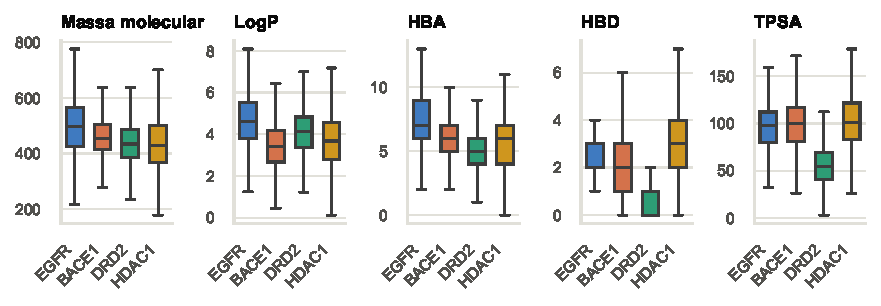
\includegraphics[width=\textwidth]{figures/feature_boxplots.pdf}
\caption{Descritores por proteína-alvo. Caixas mostram os quartis e as hastes 1,5 vez a amplitude interquartil; valores extremos foram omitidos.}
\label{fig:boxplots}
\end{figure}

TPSA, HBA e HBD são correlacionadas entre si (Spearman de 0,72 entre TPSA e HBA e de 0,69 entre TPSA e HBD), pois as três medem polaridade. Isso não prejudica a árvore, mas divide a importância entre elas. No plano LogP $\times$ TPSA (Figura~\ref{fig:scatter}), DRD2 se concentra em TPSA baixa e EGFR em LogP alto, enquanto BACE1 e HDAC1 ocupam a mesma região.

\begin{figure}[ht]
\centering
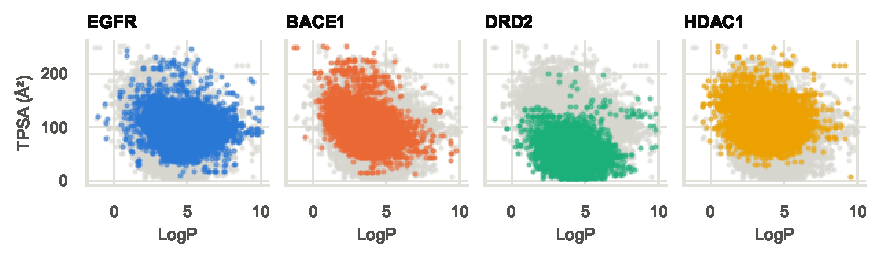
\includegraphics[width=\textwidth]{figures/logp_tpsa_by_class.pdf}
\caption{LogP $\times$ TPSA. Cada painel destaca uma classe sobre todas as moléculas (cinza).}
\label{fig:scatter}
\end{figure}

Nenhum descritor basta sozinho. Uma árvore de profundidade 3 treinada com uma única feature, em validação cruzada de 5 partes, atinge de 37,8\% (massa molecular) a 45,1\% (HBD): todas superam o piso de 29,3\%, mas nenhuma passa de 45\%. A árvore precisa combinar atributos, e o desempenho esperado com só cinco descritores globais é limitado, sobretudo entre BACE1 e HDAC1. Isso motiva as features extraídas do SMILES (Seção~\ref{sec:metodologia}).

\section{Metodologia de modelagem}\label{sec:metodologia}

Tudo foi implementado em Python com scikit-learn~\cite{pedregosa:11}. A tarefa é classificação multiclasse: prever a proteína-alvo (4 classes) das 27.476 moléculas com os cinco descritores completos.

\subsection{Conjuntos de features}

Além dos descritores, foram criadas 12 features por contagem de caracteres do SMILES, sem biblioteca de química: comprimento da cadeia; número de átomos de N, O e S; de halogênios (F, Cl, Br, I); de anéis (dígitos de fechamento dividido por 2); de ramificações (\texttt{(}); de átomos aromáticos (c, n, o, s minúsculos); de ligações duplas (\texttt{=}) e triplas (\texttt{\#}); de cargas (\texttt{+}, \texttt{-}); e de marcas de estereoquímica (\texttt{@}, \texttt{/}). Cl e Br contam como um único símbolo, para que o ``C'' de Cl não seja contado como carbono. Comparam-se três conjuntos: os 5 descritores, as 12 contagens de SMILES e os 17 atributos juntos.

\subsection{Divisão treino-teste e vazamento}\label{sec:splits}

Os dados são divididos em 80\% para treino (21.980 moléculas) e 20\% para teste (5.496), em dois esquemas. A divisão \emph{aleatória} usa amostragem estratificada comum e ignora que linhas com descritores idênticos podem cair nos dois lados. A divisão \emph{agrupada} usa o primeiro fold de um \texttt{StratifiedGroupKFold} de 5 partes, no qual todas as linhas com a mesma tupla dos cinco descritores formam um grupo que não é separado. As duas preservam a proporção das classes. A diferença entre elas mede o vazamento~\cite{kapoor:23}, ou seja, o quanto o teste aleatório premia a memorização de moléculas quase idênticas às de treino.

\subsection{Ajuste, avaliação e modelos de referência}

Para cada um dos 6 cenários (3 conjuntos de features $\times$ 2 divisões), uma busca em grade com validação cruzada de 5 partes escolhe os hiperparâmetros da árvore de decisão: critério (\texttt{gini} ou \texttt{entropy}), profundidade máxima (8, 12, 16 ou sem limite), mínimo de amostras por folha (1, 5 ou 20) e parâmetro de poda por custo-complexidade $\alpha$ (0, $10^{-4}$ ou $3\times10^{-4}$), 72 combinações. A validação interna segue a mesma disciplina da divisão externa: com treino agrupado, usa dobras agrupadas. A métrica de escolha é a acurácia. No teste, reportam-se acurácia, F1 macro (média simples do F1 das quatro classes), F1 por classe e a matriz de confusão.

Como piso e teto, usam-se no mesmo treino e teste um classificador que responde a classe majoritária, uma Random Forest de 300 árvores e um \emph{gradient boosting} baseado em histogramas (\texttt{HistGradientBoosting}), ambos sem ajuste de hiperparâmetros.

\subsection{Repetição com várias seeds}

Um único split pode ser favorável ou desfavorável por acaso. Todo o procedimento acima é repetido com 10 seeds (0 a 9), que mudam as duas divisões, as dobras da validação cruzada e a semente dos modelos. As tabelas trazem média $\pm$ desvio padrão amostral. As curvas, a árvore desenhada e a análise de erros usam a seed 42, a mesma dos notebooks do projeto. A variação das seeds cobre o sorteio da divisão, mas não a escolha dos dados: a base é a mesma em todas as repetições.

\section{Resultados e discussão}

Salvo indicação em contrário, os números são média $\pm$ desvio padrão em 10 seeds (Seção~\ref{sec:seeds}); as figuras e os exemplos de erro usam a seed 42. Acurácias e F1 estão em \%; ganhos e superestimativas são relativos.

\subsection{Vazamento por descritores repetidos}\label{sec:vazamento}

Das 27.476 moléculas, 22.699 têm uma tupla de descritores distinta e 4.777 repetem a de outra molécula (o maior grupo tem 12). Nenhum grupo mistura classes. Na divisão aleatória, \gemeas~$\pm$~\sdGemeas\% das moléculas de teste têm uma gêmea de descritores no treino, isto é, outra molécula com exatamente os mesmos cinco valores. O efeito aparece na última coluna da Tabela~\ref{tab:features}: com só os cinco descritores, a divisão aleatória superestima a acurácia em \gapDesc~$\pm$~\sdGapDesc\%, pois a árvore pode decorar as gêmeas. Com as contagens de SMILES o excesso cai para \gapSmiles\% tanto com elas sozinhas quanto com os 17 atributos, porque moléculas com os mesmos descritores têm SMILES diferentes e as contagens não são copiadas junto. A partir daqui, usa-se a divisão agrupada.

\begin{table}[ht]
\centering
\caption{Árvore de decisão no teste, por conjunto de atributos (média $\pm$ desvio em 10 seeds). Cada linha reúne dois cenários da Tabela~\ref{tab:cenarios}. Superestimativa: quanto a acurácia da divisão aleatória excede a da agrupada, em termos relativos.}
\label{tab:features}
\footnotesize
\begin{tabular}{lcccc}
\toprule
Atributos & \shortstack{Acurácia\\aleatória} & \shortstack{Acurácia\\agrupada} & \shortstack{F1 macro\\agrupado} & \shortstack{Superestimativa\\(pontos)} \\
\midrule
Descritores (5) & 0,812 $\pm$ 0,005 & 0,771 $\pm$ 0,008 & 0,770 $\pm$ 0,008 & 4,1 $\pm$ 0,9 \\
SMILES (12) & 0,889 $\pm$ 0,004 & 0,876 $\pm$ 0,006 & 0,873 $\pm$ 0,006 & 1,3 $\pm$ 0,9 \\
Ambos (17) & 0,908 $\pm$ 0,003 & 0,894 $\pm$ 0,004 & 0,893 $\pm$ 0,004 & 1,4 $\pm$ 0,4 \\
\bottomrule
\end{tabular}

\end{table}

\subsection{Efeito dos atributos de SMILES}

Na divisão agrupada, os cinco descritores dão acurácia de \accGrupDesc~$\pm$~\sdGrupDesc\%. As 12 contagens de SMILES sozinhas chegam a \accGrupSmiles~$\pm$~\sdGrupSmiles\%, um ganho relativo de \ganhoSmiles\%. Os 17 atributos juntos chegam a \accGrupAmbos~$\pm$~\sdGrupAmbos\% (F1 macro de \fscoreGrupAmbos\%), um ganho relativo de \ganhoAmbos\% sobre os descritores, muito acima da variação entre seeds. Contar letras de uma cadeia de texto carrega mais informação sobre a molécula, como o número de anéis aromáticos e de halogênios, do que cinco propriedades globais. Na seed 42, a árvore escolhida acerta 89,7\%, dentro da faixa de \faixaMin\% a \faixaMax\% observada nas 10 seeds.

\subsection{Profundidade e poda}

A busca em grade escolheu a entropia como critério e nenhum limite de profundidade nos seis cenários, e só ativou a poda quando os atributos eram apenas os descritores: com cerca de 22 mil linhas de treino, a regra de parada da própria árvore já fica perto do ideal. A Figura~\ref{fig:curvas}a mostra o motivo. A acurácia de treino chega a 100\% na profundidade 25, enquanto a de validação estaciona em torno de 87\% a partir da profundidade 16. A poda por custo-complexidade (Figura~\ref{fig:curvas}b) reduz a árvore de 2.054 para 899 folhas com $\alpha = 10^{-4}$ sem perder acurácia de validação (87,0\% para 87,2\%); acima de $10^{-3}$ a poda passa a custar acurácia, e com $\alpha = 10^{-2}$ sobram 8 folhas e 66,5\%.

\begin{figure}[ht]
\centering
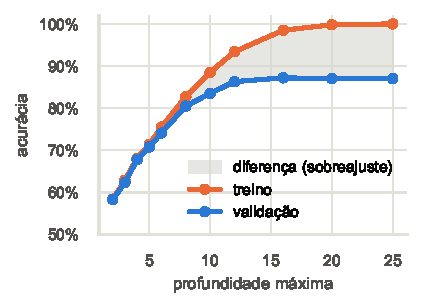
\includegraphics[width=.49\textwidth]{figures/depth_curve.pdf}\hfill
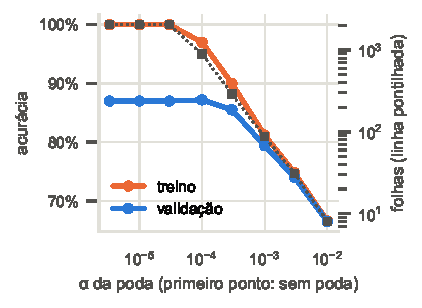
\includegraphics[width=.49\textwidth]{figures/pruning_curve.pdf}
\caption{Acurácia de treino e de validação (seed 42, divisão agrupada, 17 atributos). (a) Por profundidade máxima. (b) Por $\alpha$ da poda, com o número de folhas na escala da direita (linha pontilhada); o primeiro ponto é $\alpha=0$.}
\label{fig:curvas}
\end{figure}

\subsection{O que a árvore aprendeu}

A árvore escolhida tem 1.854 folhas e 24 níveis, grande demais para ser desenhada. As primeiras camadas, porém, são legíveis. A raiz divide por TPSA (limiar de 67,9) e o ramo de TPSA baixa tem 69\% de DRD2, como a análise exploratória antecipava. Em seguida vêm o número de átomos aromáticos, um atributo do SMILES, e depois HBD, número de anéis, comprimento do SMILES e número de halogênios. Descritores e contagens se misturam já no topo. A Figura~\ref{fig:import} confirma o quadro: TPSA e o número de átomos aromáticos lideram nas duas medidas de importância, seguidos por HBD e por um bloco de contagens (átomos de N, halogênios, estereoquímica, anéis) acima de LogP e HBA. A importância por permutação, medida no teste, dá mais peso às contagens do que a de impureza.

\begin{figure}[ht]
\centering
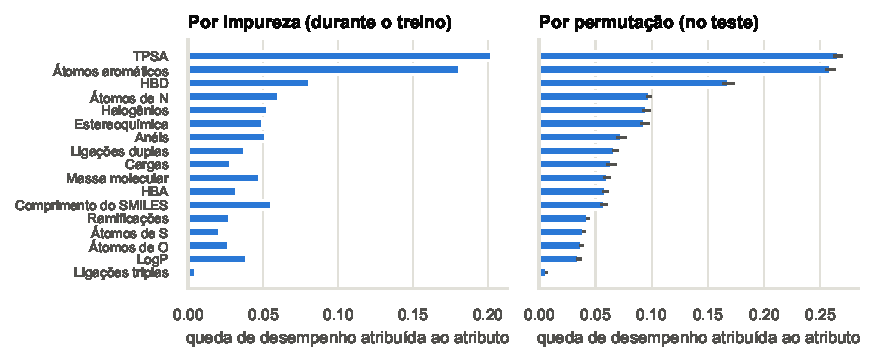
\includegraphics[width=\textwidth]{figures/feature_importances.pdf}
\caption{Importância dos atributos da árvore escolhida (seed 42). À esquerda, a redução de impureza acumulada nos nós que usam o atributo, durante o treino. À direita, a queda de acurácia no teste quando os valores do atributo são embaralhados (permutação).}
\label{fig:import}
\end{figure}

\subsection{Erros e limites da árvore}

Entre as classes, BACE1 e DRD2 são as mais fáceis (F1 de \fscoreBACEone\% e \fscoreDRDtwo\%), seguidas de EGFR (\fscoreEGFR\%) e HDAC1 (\fscoreHDACone\%), a mais difícil. Na seed 42, o par HDAC1 $\leftrightarrow$ EGFR, nos dois sentidos, soma 28,7\% dos 568 erros (Figura~\ref{fig:erros}a), e 7,9\% das moléculas de HDAC1 viram EGFR. Os erros não ocupam uma região do espaço de atributos: nenhum dos 17 atributos desloca a mediana entre acertos e erros em mais de meio intervalo interquartil. Entre seis exemplos de HDAC1 lidos como EGFR, dois contêm a mesma subestrutura, o grupo de átomos C(=O)NO. A árvore não a distingue: contagens de caracteres dizem quantos oxigênios e nitrogênios existem, mas não como estão ligados.

A árvore também não sabe quando erra. Sem poda, toda folha é pura, então a probabilidade de classe estimada pela árvore é 100\% nas 5.496 previsões de teste, embora 10,3\% estejam erradas. A curva de aprendizado (Figura~\ref{fig:erros}b) mostra a outra limitação: o treino fica em 100\% e a validação sobe de 61,5\% (879 linhas) para 87,0\% (17.584) sem se achatar, de modo que mais moléculas provavelmente renderiam mais acurácia.

\begin{figure}[ht]
\centering
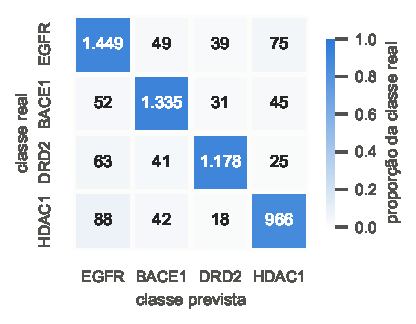
\includegraphics[width=.44\textwidth]{figures/confusion_matrix.pdf}\hfill
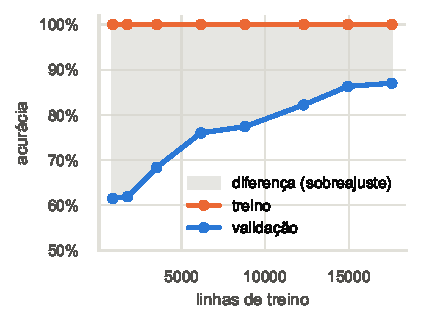
\includegraphics[width=.52\textwidth]{figures/learning_curve.pdf}
\caption{Seed 42, divisão agrupada, 17 atributos. (a) Matriz de confusão no teste: cor pela proporção da classe real, número em contagem. (b) Curva de aprendizado: acurácia por tamanho do conjunto de treino.}
\label{fig:erros}
\end{figure}

\subsection{Comparação com modelos de referência}

A Tabela~\ref{tab:referencia} situa a árvore entre um piso e um teto. Responder sempre EGFR, a classe majoritária, dá \accMaj\% de acurácia, que é a proporção de EGFR na base. A Random Forest~\cite{breiman:01} chega a \accRF~$\pm$~\sdRF\% e o \emph{gradient boosting} a \accHGB~$\pm$~\sdHGB\%, enquanto a árvore única acerta \accArvore~$\pm$~\sdArvore\%: a Random Forest supera a árvore em \ganhoRF\% (relativo). Esse ganho é o preço da interpretabilidade: a árvore responde por que uma molécula foi classificada como DRD2 com um caminho de perguntas sobre TPSA e contagens, enquanto os conjuntos não têm regras legíveis.

\begin{table}[ht]
\centering
\caption{Árvore e modelos de referência na divisão agrupada, com os 17 atributos (média $\pm$ desvio em 10 seeds).}
\label{tab:referencia}
\footnotesize
\begin{tabular}{lcc}
\toprule
Modelo & Acurácia & F1 macro \\
\midrule
Classe majoritária & 0,293 $\pm$ 0,000 & 0,113 $\pm$ 0,000 \\
Árvore de decisão & 0,894 $\pm$ 0,004 & 0,893 $\pm$ 0,004 \\
Random Forest (300 árvores) & 0,952 $\pm$ 0,003 & 0,951 $\pm$ 0,003 \\
HistGradientBoosting & 0,948 $\pm$ 0,003 & 0,947 $\pm$ 0,003 \\
\bottomrule
\end{tabular}

\end{table}

\section{Limitações}

O agrupamento por descritores idênticos não cobre famílias de moléculas muito parecidas entre si, que continuam espalhadas entre treino e teste; as contagens de SMILES permitem decorar essas famílias. Dividir por família (esqueleto molecular) controlaria isso, mas exige uma biblioteca de química. Por isso a acurácia de \accGrupAmbos\% ainda é otimista para moléculas realmente novas.

O modelo escolhe sempre uma entre quatro classes: não existe a opção ``nenhuma das quatro'', então ele não sabe dizer que uma molécula não pertence a nenhum dos alvos. As 10 seeds variam o sorteio da divisão, mas os dados são os mesmos, de modo que o desvio padrão não mede a incerteza para dados novos, e não há validação externa. A Random Forest e o \emph{gradient boosting} usam hiperparâmetros padrão, e o teto que representam pode estar subestimado. Por fim, as 238 moléculas sem descritores (0,86\%) foram descartadas, em sua maioria muito grandes, e as probabilidades da árvore não são calibradas.

\section{Conclusão e trabalhos futuros}

Reconstruímos do ChEMBL\_37 uma base de 27.714 moléculas ativas contra EGFR, BACE1, DRD2 e HDAC1 e treinamos uma árvore de decisão para prever o alvo. Com divisão agrupada, os cinco descritores físico-químicos dão acurácia de 0,771; acrescentar 12 contagens de caracteres do SMILES a leva a 0,894~$\pm$~0,004, e as contagens sozinhas já chegam a 0,876. A divisão aleatória superestima o resultado em 1,3 a 4,1 pontos porque cerca de um quarto das moléculas de teste tem gêmea de descritores no treino. TPSA e o número de átomos aromáticos são os atributos mais importantes, e o par HDAC1--EGFR concentra 28,7\% dos erros. A Random Forest chega a 0,952, cerca de 6 pontos acima da árvore, que em troca oferece regras legíveis.

Quatro caminhos seguem do que foi visto. Fingerprints estruturais, calculados com uma biblioteca de química, enxergariam subestruturas como o hidroxamato, que as contagens não veem. Uma divisão por esqueleto molecular daria uma estimativa menos otimista para moléculas novas. A curva de aprendizado ainda sobe, o que sugere buscar mais dados no ChEMBL, com outros alvos ou um limiar de atividade mais frouxo. Por fim, podar a árvore ou usar um conjunto de árvores daria probabilidades calibradas, e incluir moléculas inativas faria o modelo servir também à triagem.


\bibliographystyle{sbc}
\bibliography{refs}

\end{document}
